\documentclass[aspectratio=169]{beamer}
\usetheme[noborder]{Jacquenetta}  % default accent is jqblue; drop the frame border for space

\usepackage[T1]{fontenc}
\usepackage[utf8]{inputenc}
\usepackage{amsmath,amssymb}
\usepackage{booktabs}
\usepackage{graphicx}
\usepackage{listings}
\usepackage{xcolor}

% Figures live one level up, shared with the manual/report.
\graphicspath{{../img/}}

% --- Compact code style for GLSL / C++ snippets --------------------------------
% language=C++ is what makes listings actually tokenize (identify comments,
% strings and keywords); without it every token falls through to basicstyle and
% renders black. A second keyword class colours the GLSL/CUDA/GL identifiers that
% the C++ language table doesn't know about.
\lstdefinestyle{gol}{%
  language=C++,
  basicstyle=\ttfamily\scriptsize\color{jqdark},
  keywordstyle=\color{jqblue}\bfseries,
  keywordstyle=[2]\color{jqorange}\bfseries,
  commentstyle=\color{jqgray}\itshape,
  stringstyle=\color{jqgreen},
  morekeywords=[2]{%
    vec2,vec3,vec4,ivec2,ivec3,uvec2,mat3,mat4,uniform,usampler2D,sampler2D,%
    texelFetch,texture,fract,floor,mix,clamp,dot,gl_Position,gl_VertexID,%
    gl_FragColor,cudaGraphicsGLRegisterBuffer,cudaGraphicsMapResources,%
    cudaGraphicsResourceGetMappedPointer,cudaMemcpy,cudaGraphicsUnmapResources,%
    cudaGraphicsRegisterFlagsWriteDiscard,cudaMemcpyDeviceToDevice,%
    glTexImage2D,glTexSubImage2D,GL_R8UI,GL_RED_INTEGER,GL_UNSIGNED_BYTE,%
    GL_TEXTURE_2D,palette,cellAt},
  showstringspaces=false,
  columns=fullflexible,
  keepspaces=true,
  breaklines=true,
  tabsize=2,
  aboveskip=1pt, belowskip=1pt,
}
\lstset{style=gol}

% === Metadata ===================================================
\title{El Juego de la Vida en tiempo real}
\subtitle{Interoperabilidad CUDA\,$\leftrightarrow$\,OpenGL y shaders}
\author{Matías Saavedra}
\institute{CC7515-1 --- Computación en GPU \quad\textbullet\quad U. de Chile}
\date{Tarea 3 --- Interop / Shaders \quad\textbullet\quad Julio 2026}

\begin{document}

% ============================================================ 1. Título
\titleframe

% ============================================================ 2. Problema
\begin{frame}{El problema}
    \small
    Reutilizamos el \textbf{Juego de la Vida} de la Tarea~2 --- variante
    \textbf{HighLife} (\texttt{B36/S23}): una célula muerta \emph{nace} con 3
    \textbf{o} 6 vecinos; una viva sobrevive con 2 o 3.

    \vspace{0.2cm}
    \begin{columns}[T]
        \begin{column}{0.55\textwidth}
            \begin{problock}{El reto de esta tarea}
                El tablero se calcula \textbf{en la GPU} (kernel CUDA). Dibujarlo
                de lo \emph{natural} --- copiarlo a la RAM y subirlo a OpenGL cada
                frame --- cruza el bus \textbf{PCIe} dos veces por generación.
            \end{problock}
        \end{column}
        \begin{column}{0.42\textwidth}
            \begin{highlightbox}
                \textbf{Objetivo:} mostrar el tablero \textbf{sin sacarlo de la
                GPU}, coloreado por un \emph{fragment shader}, de forma interactiva.
            \end{highlightbox}
        \end{column}
    \end{columns}

    \vspace{0.2cm}
    \textbf{Idea clave (interop):} lo que produce CUDA y lo que consume OpenGL
    viven en \emph{la misma} memoria de video $\Rightarrow$ si lo compartimos, el
    render es \textbf{copia cero} (\emph{zero-copy}).
\end{frame}

% ============================================================ 3. Arquitectura
\begin{frame}{Arquitectura: un front-end sobre el mismo núcleo}
    \begin{columns}[T]
        \begin{column}{0.47\textwidth}
            \footnotesize
            \texttt{gol\_gui} es un ejecutable aparte del \texttt{gol} headless:
            \textbf{Qt es dueña del loop}, así que no reusa el bucle de
            \texttt{main.cpp}.

            \vspace{0.1cm}
            \begin{itemize}\footnotesize
                \item \texttt{GolGlWidget} conduce cualquier
                      \texttt{ISimEngine} (CPU o CUDA).
                \item Presenta el tablero por \textbf{uno de dos caminos},
                      elegido al iniciar.
                \item \texttt{CudaGlInterop} es el puente CUDA\,$\leftrightarrow$\,GL.
            \end{itemize}

            \begin{block}{Patrón}
                \footnotesize\emph{Strategy}: motor y camino de presentación
                intercambiables; el shader no cambia.
            \end{block}
        \end{column}
        \begin{column}{0.52\textwidth}
            \centering
            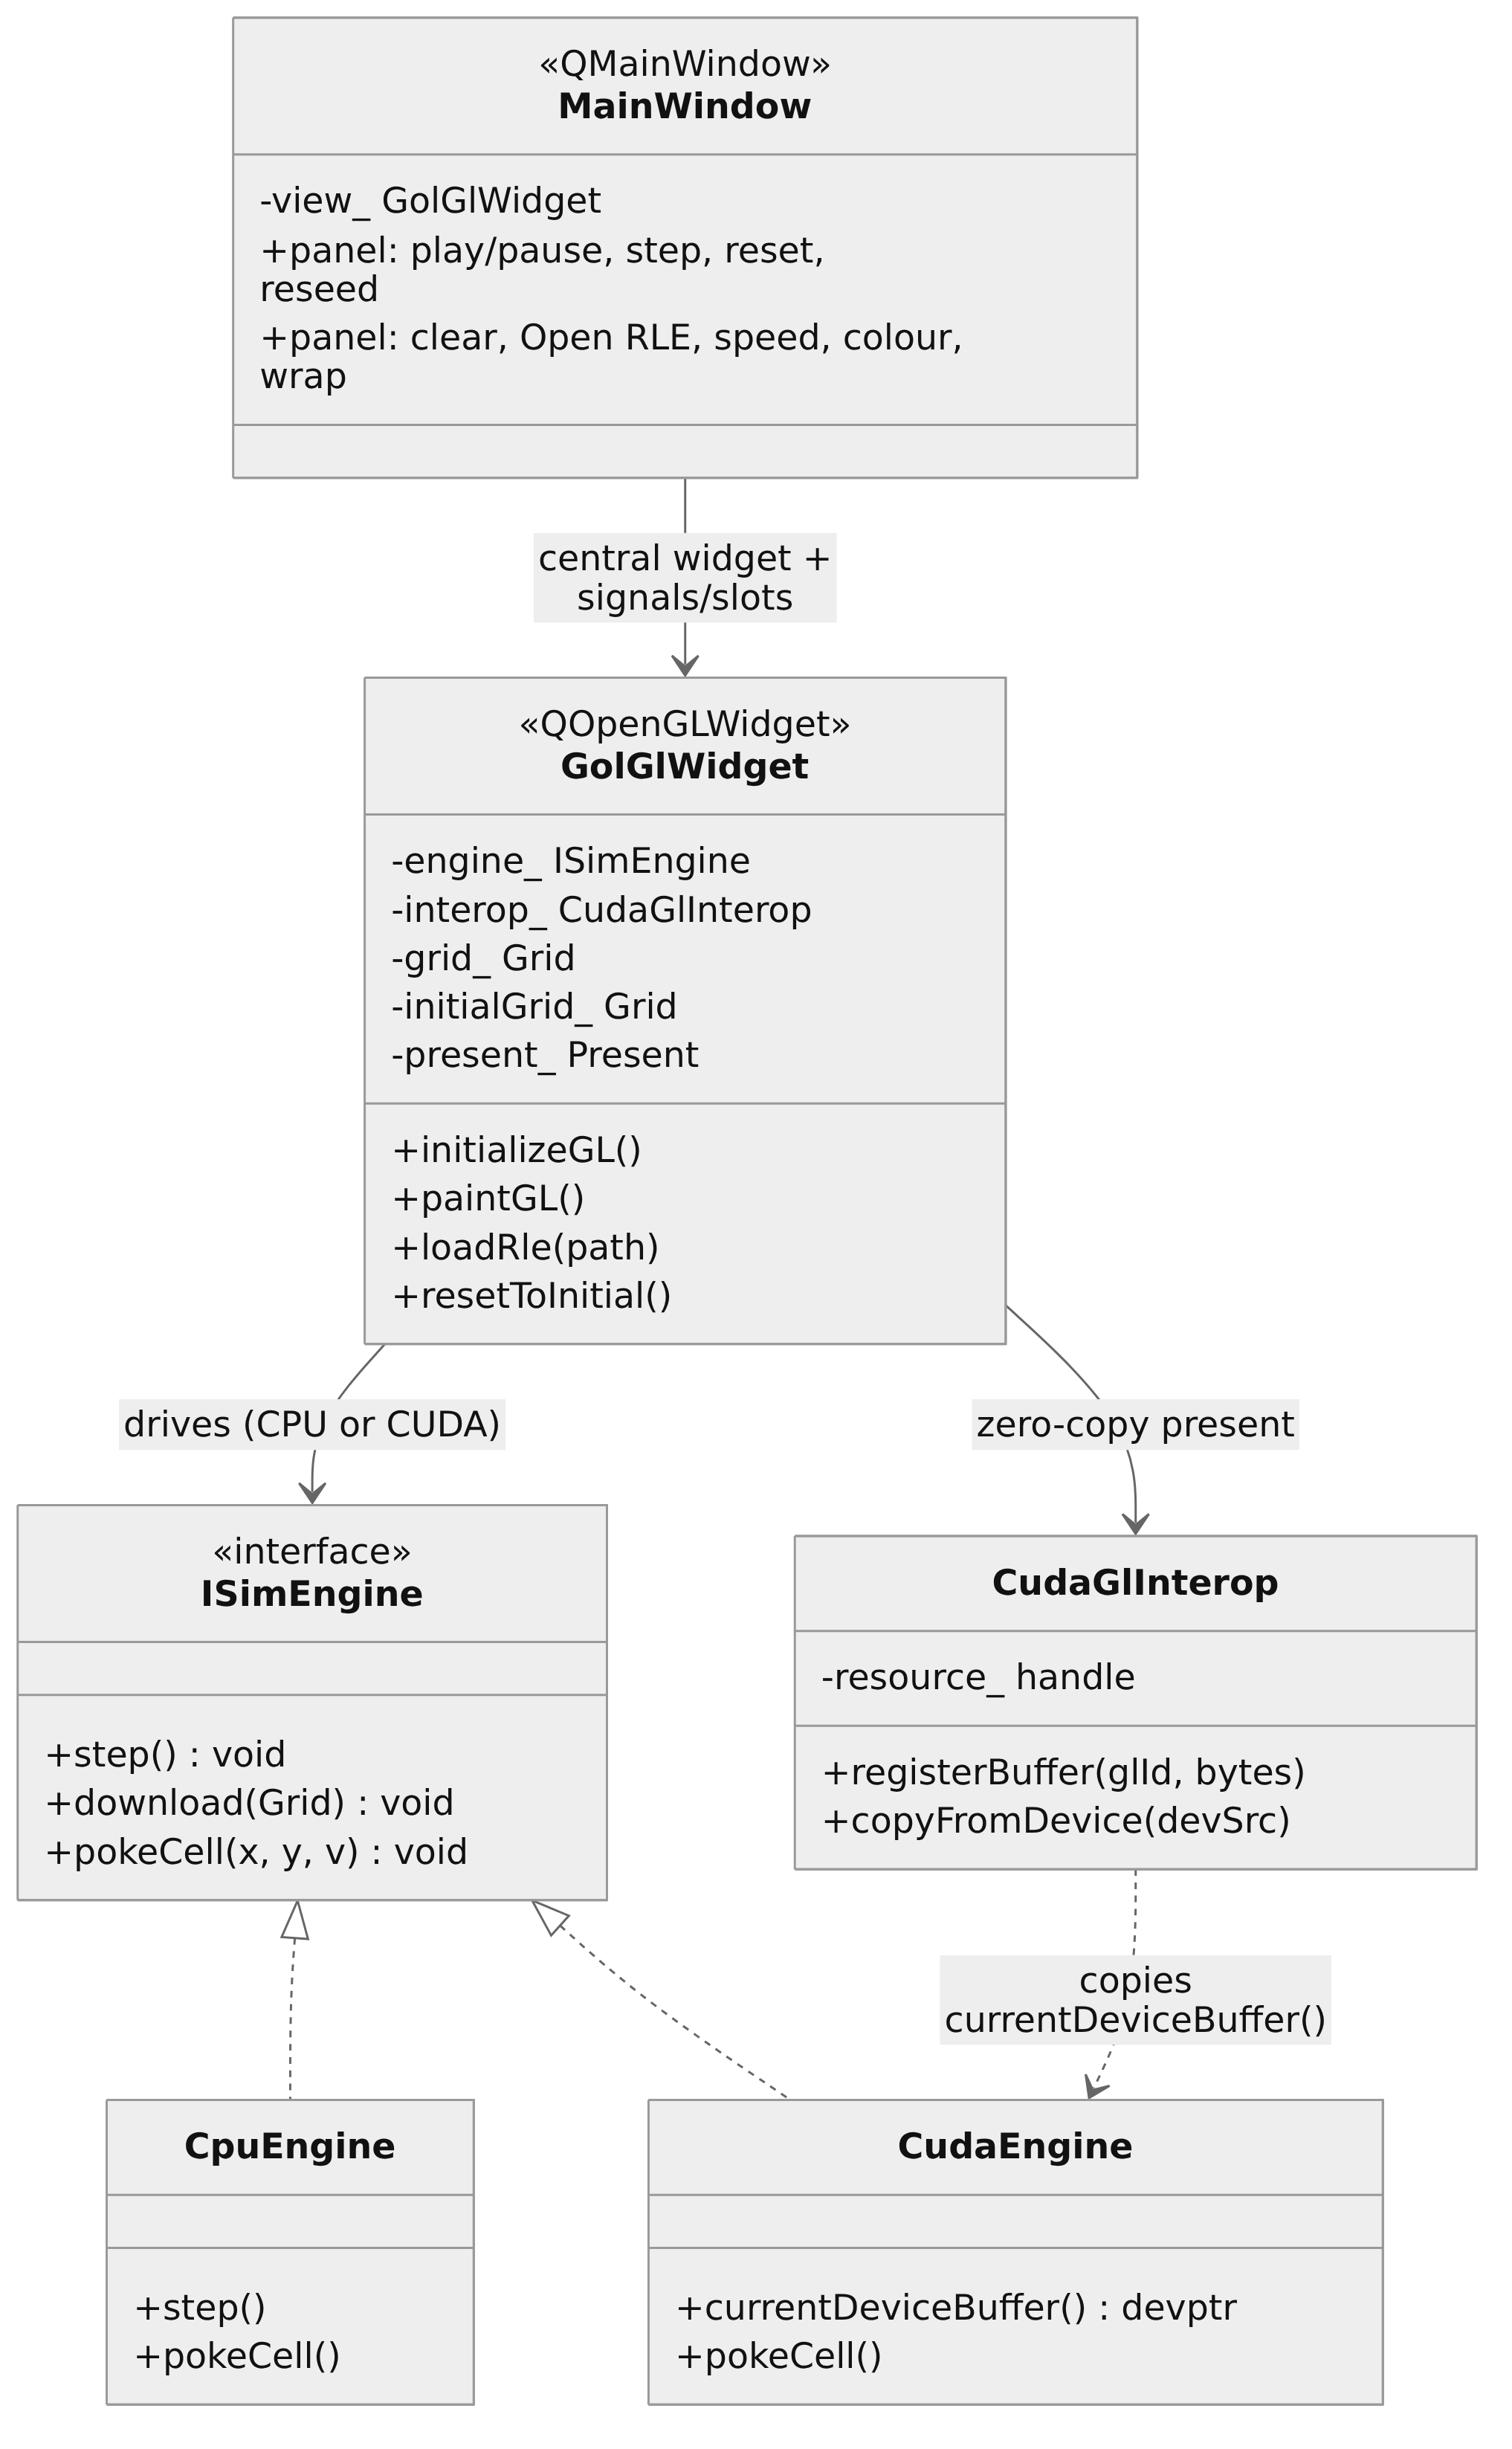
\includegraphics[height=0.74\textheight]{gui_architecture.png}
        \end{column}
    \end{columns}
\end{frame}

% ============================================================ 4. Interop (corazón)
\begin{frame}[fragile]{El corazón: interop CUDA\,$\leftrightarrow$\,OpenGL}
    \centering
    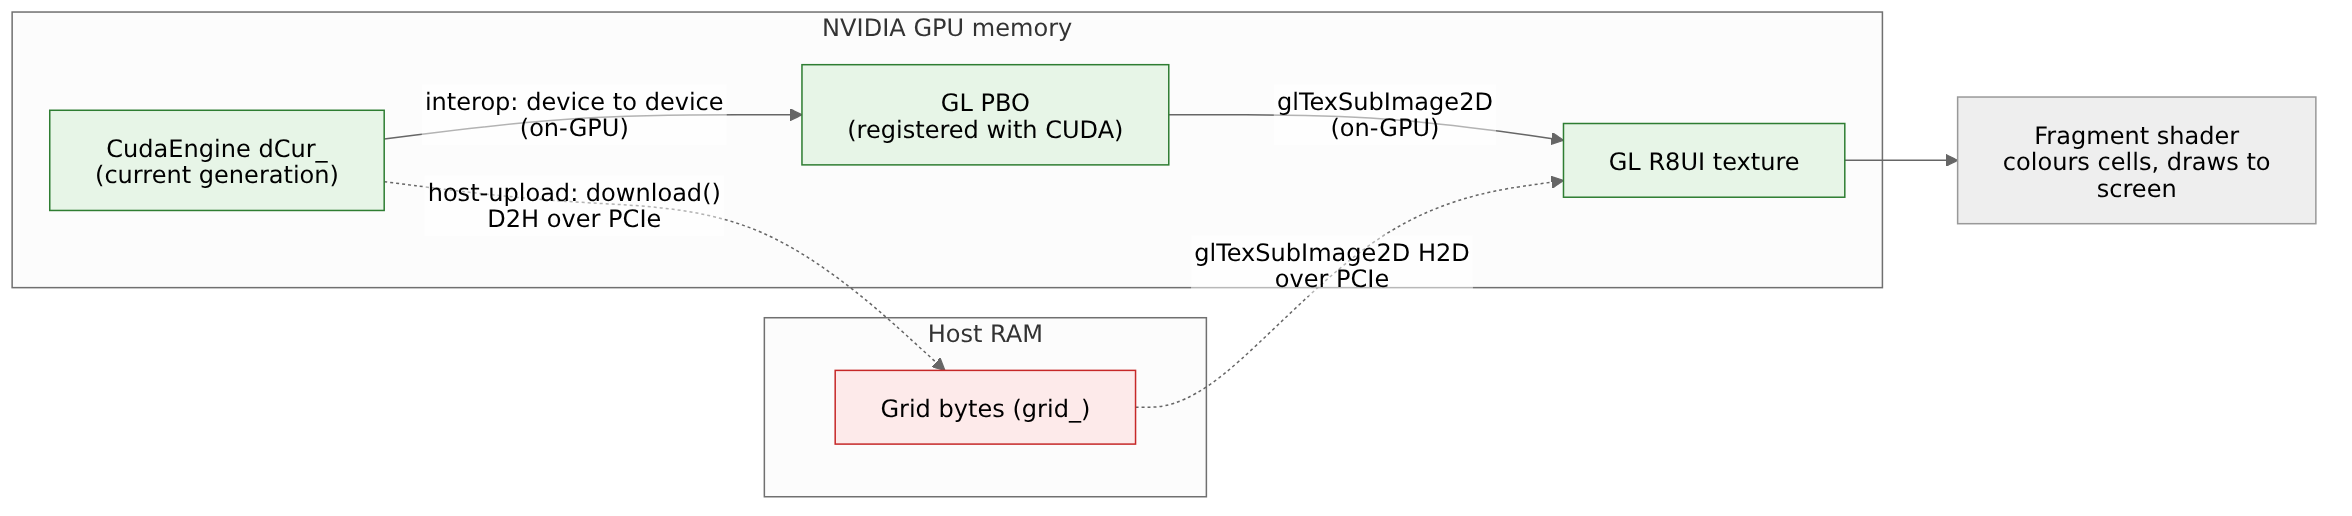
\includegraphics[width=0.80\textwidth]{gui_dataflow.png}

    \begin{columns}[T]
        \begin{column}{0.5\textwidth}
            \scriptsize
            \textbf{Una vez} (al iniciar): registrar un \emph{Pixel Buffer Object}
            de GL con CUDA.
\begin{lstlisting}
cudaGraphicsGLRegisterBuffer(&res, pbo,
    cudaGraphicsRegisterFlagsWriteDiscard);
\end{lstlisting}
        \end{column}
        \begin{column}{0.5\textwidth}
            \scriptsize
            \textbf{Cada frame:} map $\to$ copia \emph{device-to-device} $\to$
            unmap. Nada cruza PCIe.
\begin{lstlisting}
cudaGraphicsMapResources(1, &res, 0);
cudaGraphicsResourceGetMappedPointer(
    &dPtr, &n, res);
cudaMemcpy(dPtr, cuda.currentDeviceBuffer(),
           n, cudaMemcpyDeviceToDevice);
cudaGraphicsUnmapResources(1, &res, 0);
\end{lstlisting}
        \end{column}
    \end{columns}
    {\scriptsize Luego \texttt{glTexSubImage2D} lleva el PBO a la textura (también
    \emph{on-GPU}). Contexto GL en otra GPU $\Rightarrow$ \textbf{fallback}
    \emph{host-upload}.}
\end{frame}

% ============================================================ 5. Tablero en GPU
\begin{frame}[fragile]{El tablero como textura en la GPU}
    \begin{columns}[T]
        \begin{column}{0.53\textwidth}
            \footnotesize
            El tablero es \textbf{1 byte por celda} (0 muerta, 1 viva), guardado en
            una textura \textbf{\texttt{GL\_R8UI}} (enteros sin signo, un canal).

            \vspace{0.15cm}
            \begin{itemize}\footnotesize
                \item Se lee \emph{exacto} con \texttt{usampler2D} +
                      \texttt{texelFetch}: los enteros no se interpolan.
                \item \texttt{GL\_NEAREST}: cada celda es un cuadrado nítido.
                \item El motor CUDA hace \emph{ping-pong} de dos buffers; el shader
                      lee siempre \texttt{currentDeviceBuffer()}.
            \end{itemize}

            \vspace{0.1cm}
            \begin{block}{Por qué entera}
                Evita que el hardware \emph{promedie} celdas: 1 texel $=$ 1 célula.
            \end{block}
        \end{column}
        \begin{column}{0.45\textwidth}
\begin{lstlisting}
// creacion de la textura
glTexImage2D(GL_TEXTURE_2D, 0,
    GL_R8UI, cols, rows, 0,
    GL_RED_INTEGER,
    GL_UNSIGNED_BYTE, nullptr);

// en el shader (GLSL)
uniform usampler2D uBoard;
int alive =
   int(texelFetch(uBoard,cell,0).r);
\end{lstlisting}
        \end{column}
    \end{columns}
\end{frame}

% ============================================================ 6. Vertex shader
\begin{frame}[fragile]{Vertex shader: un triángulo que cubre la pantalla}
    \begin{columns}[T]
        \begin{column}{0.5\textwidth}
            \footnotesize
            No hay geometría del tablero que enviar: dibujamos \textbf{un solo
            triángulo} que tapa la pantalla. Sus vértices salen de
            \texttt{gl\_VertexID} --- \textbf{sin VBO}.
\begin{lstlisting}
// display.vert (3 vertices, 1 draw)
void main() {
  vec2 v[3] = vec2[3](
    vec2(-1,-1), vec2(3,-1), vec2(-1,3));
  gl_Position =
    vec4(v[gl_VertexID], 0.0, 1.0);
}
\end{lstlisting}
        \end{column}
        \begin{column}{0.5\textwidth}
            \footnotesize
            Todo el trabajo ocurre \textbf{por pixel}. Cada pixel se convierte en
            una \emph{celda} invirtiendo la misma cámara (zoom + pan) que usa el
            ratón:
\begin{lstlisting}
// pixel de pantalla -> celda
vec2 boardF = uCenter +
    (screen - 0.5*uViewSize) / uScale;
ivec2 cell = ivec2(floor(boardF));
\end{lstlisting}
            \begin{highlightbox}
                \footnotesize
                \texttt{uScale} $=$ pixeles por celda (rueda);\;
                \texttt{uCenter} $=$ celda al centro (arrastre).
            \end{highlightbox}
        \end{column}
    \end{columns}
\end{frame}

% ============================================================ 7. Fragment shader
\begin{frame}[fragile]{Fragment shader: cómo se colorea cada celda}
    \begin{columns}[T]
        \begin{column}{0.52\textwidth}
            \footnotesize
            Un \texttt{uniform} elige el \textbf{modo}; otro la \textbf{paleta}.
            Todo se resuelve leyendo la textura:
            \begin{description}\footnotesize
                \item[Binario] viva $=$ color caliente, muerta oscura.
                \item[Vecinos] cuenta los 8 vecinos con \texttt{texelFetch}
                      (gratis) y mapea $0..8$ a la rampa.
                \item[Edad] colorea según generaciones vividas (2\textsuperscript{a}
                      textura de edad).
            \end{description}
            5 paletas: phosphor, amber, grayscale, magma, ice.
        \end{column}
        \begin{column}{0.48\textwidth}
\begin{lstlisting}
if (uColorMode == 1) {       // vecinos
  int n = cellAt(cell+ivec2(-1,-1))
      +...+ cellAt(cell+ivec2(1,1));
  col = palette(uPalette, n/8.0);
} else {                     // binario
  col = (alive==1)
    ? palette(uPalette,1.0) : DEAD;
}
// lineas de grilla al acercar
if (uScale >= 4.0) {
  vec2 f = fract(boardF);
  col *= mix(0.35, 1.0, ...);
}
\end{lstlisting}
        \end{column}
    \end{columns}
\end{frame}

% ============================================================ 8. Qt
\begin{frame}[fragile]{Qt: la ventana, el loop y los controles}
    \begin{columns}[T]
        \begin{column}{0.52\textwidth}
            \footnotesize
            \textbf{Qt es dueña del bucle} (\texttt{QApplication::exec()}); por eso
            el visor es un \emph{front-end}, no un \texttt{IRenderer}.
            \begin{itemize}\footnotesize
                \item \texttt{GolGlWidget} : \texttt{QOpenGLWidget} ---
                      \texttt{initializeGL / paintGL / resizeGL}.
                \item \texttt{QTimer} a $\sim$60\,Hz llama \texttt{update()}:
                      repinta y avanza una generación.
                \item \texttt{MainWindow} : \texttt{QMainWindow} con un \textbf{panel
                      dockable} (play, step, reset, RLE, color, paleta, wrap).
            \end{itemize}
        \end{column}
        \begin{column}{0.46\textwidth}
            \begin{block}{Señales y slots}
                \footnotesize Los botones se conectan a \emph{slots} del widget.
            \end{block}
\begin{lstlisting}
connect(playBtn, &QPushButton::toggled,
        view, &GolGlWidget::setPlaying);
\end{lstlisting}
            \begin{highlightbox}
                \footnotesize
                \textbf{Interacción:} rueda $=$ zoom, arrastre medio/dcho.\ $=$
                pan, arrastre izq.\ $=$ pintar (Shift borra); teclas
                \texttt{space/S/R/C/I/F/P}.
            \end{highlightbox}
        \end{column}
    \end{columns}
\end{frame}

% ============================================================ 9. Problemas
\begin{frame}{Problemas encontrados y cómo se resolvieron}
    \footnotesize
    \begin{block}{1. Optimus: el contexto GL cae en la iGPU Intel}
        En este portátil híbrido OpenGL usa por defecto la Intel; ahí el interop
        con CUDA (NVIDIA) \textbf{falla}. \alert{Solución:} detectar el error y caer
        a \emph{host-upload} sin romperse; \texttt{scripts/run\_gui.sh} fija
        variables PRIME para forzar el contexto en la NVIDIA (camino zero-copy).
    \end{block}
    \begin{block}{2. Una célula recién pintada desaparecía}
        \alert{Solución:} cada frame \textbf{presenta y luego avanza}
        (present-then-step): lo dibujado se ve el frame en que se pinta, y sólo
        después evoluciona.
    \end{block}
    \begin{block}{3. El heatmap de edad no debe frenar el camino rápido}
        El buffer de edad es \emph{host-side} y sólo se actualiza \textbf{cuando ese
        modo está activo}; los demás modos y el interop siguen zero-copy.
    \end{block}
\end{frame}

% ============================================================ 10. Repaso T2 -> T3
\begin{frame}{De la Tarea 2 a la Tarea 3: qué se entregó y qué cambió}
    \footnotesize
    \begin{columns}[T]
        \begin{column}{0.5\textwidth}
            \begin{block}{Tarea 2 --- lo entregado}
                \scriptsize
                Juego de la Vida (variante \texttt{B36/S23}) en \textbf{tres motores}:
                \begin{itemize}\scriptsize
                    \item \textbf{CPU} secuencial + paralelo (\texttt{std::barrier}).
                    \item \textbf{CUDA} y \textbf{OpenCL}: 1 hilo/celda, \emph{ping-pong}
                          en el \emph{device}, kernels global y \emph{shared/local}.
                    \item Verificados \textbf{bit a bit} vs.\ el oráculo CPU (y Golly).
                \end{itemize}
                Métrica: \textbf{celdas/s}; \alert{$\sim$35--37\,Gcel/s} ($\sim$240$\times$ CPU).
            \end{block}
        \end{column}
        \begin{column}{0.5\textwidth}
            \begin{block}{Tarea 3 --- lo que cambió}
                \scriptsize
                \textbf{El núcleo no se tocó}: \texttt{Grid}, \texttt{LifeRules},
                \texttt{ISimEngine} y los motores se reusan \emph{tal cual}.
                \begin{itemize}\scriptsize
                    \item \textbf{Nuevo} front-end \texttt{gol\_gui} (Qt), \emph{no} un
                          \texttt{IRenderer}: Qt es dueña del loop.
                    \item \textbf{Nuevo} \texttt{CudaGlInterop} (zero-copy) $+$ shaders
                          GLSL que colorean cada celda $+$ fallback \emph{host-upload}.
                    \item \texttt{ISimEngine::pokeCell} para pintar con el ratón.
                \end{itemize}
            \end{block}
        \end{column}
    \end{columns}
    \begin{highlightbox}
        \footnotesize
        \textbf{La clave:} el patrón \emph{Strategy} de la Tarea~2 hizo que sumar un
        visor en tiempo real fuera casi todo \textbf{aditivo} --- la simulación no se
        modificó.
    \end{highlightbox}
\end{frame}

\end{document}
